\documentclass[12pt]{article}
\setlength{\oddsidemargin}{0in}
\setlength{\evensidemargin}{0in}
\setlength{\textwidth}{6.5in}
\setlength{\parindent}{0in}
\setlength{\parskip}{\baselineskip}

\usepackage{amsmath,amsfonts,amssymb,bm,graphicx,pgfplots,framed,dsfont}
\usepackage[scale=0.75,top=1cm,bottom=3cm]{geometry}

\begin{document}

\textbf{Minh Anh Nguyen }\\
\textbf{Calculus 1\hfill Written HW-2}

\hrulefill

Section 1.5:

\begin{enumerate}
%--%

\item 
Explain in your own words what is meant by the equation
    \[ \lim_{x \to 2 } f(x) = 5\]
Is it possible for this statement to be true and yet f(2) = 3? Explain.\\
  \textbf{Answer:} \\~\\
  \noindent\fbox{
    \parbox{410px}{
        The equation indicates that as x approaches 2, the function of x will approach 5.\\~\\
        It is possible for this statement to be true and $f(2) = 3$, because it only implies that as 
        x gets very close to 2, the function value f(x) gets very close to 5. It doesn't require f(x) to actually be 5.
    }
  }
  
\end{enumerate}

\begin{enumerate}
\setcounter{enumi}{4}
    \item For the function $f$ whose graph is given, state the value of each quantity, if it exists. If it does not exist, explain why.
    \begin{center}
    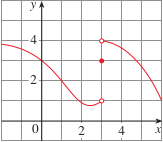
\includegraphics{Images/Image-0.png}
    \end{center}
    \begin{enumerate}
        \item \[ \boxed{\lim_{x \to 1} f(x) = 2}\]
        \item \[ \boxed{\lim_{x \to 3^-} f(x) = 1}\]
        \item \[ \boxed{\lim_{x \to 3^+} f(x) = 4}\]
        \item \[ \boxed{\lim_{x \to 3} f(x) \text{ does not exist.}}\]
        \item \[ \boxed{f(3) = 3}\]
    \end{enumerate}
\end{enumerate}

\newpage
\begin{enumerate}
\setcounter{enumi}{6}
    \item For the function $f$ whose graph is shown, find a number $a$ that satisfies the given description.
    \begin{center}
        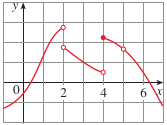
\includegraphics{Images/Image-1.png}
    \end{center}
    \begin{enumerate}
        \item $\displaystyle{\lim_{x \to a} g(x)}$ does not exist but g(a) is defined.\\~\\
        \textbf{Answer:} $\boxed{a = 4}$\\
        \item $\displaystyle{\lim_{x \to a} g(x)}$ exists but g(a) is not defined.\\~\\
        \textbf{Answer:} $\boxed{a = 5}$\\
        \item $\displaystyle{\lim_{x \to a^-} g(x)}$ and $\displaystyle{\lim_{x \to a^+} g(x)}$ both exist but $\displaystyle{\lim_{x \to a} g(x)}$ does not exist.\\~\\
        \textbf{Answer:} $\boxed{a = 2}$ and $\boxed{a = 4}$\\
        \item $\displaystyle{\lim_{x \to a^+} g(x) = g(a)}$ but $\displaystyle{\lim_{x \to a^-} g(x) \neq g(a)}$.\\~\\
        \textbf{Answer:} $\boxed{a = 4}$\\
    \end{enumerate}
\end{enumerate}

\newpage
\begin{enumerate}
\setcounter{enumi}{10}
    \item Sketch the graph of the function and use it to determine the values of $a$ for which $\displaystyle{\lim_{x \to a} f(x)}$ exists.
        \[ f(x) = \left \{ \begin{array}{l}
      \cos x \text{ if } x \leqslant 0 \\
    1 - x \text{ if } 0 < x < 1 \\
    {\displaystyle \frac{1}{x}} \text{ if } x \geqslant 1 \end{array} \right.  \] 
\\~\\
\textbf{Answer:}
      
    \begin{figure}[!h]      
    \begin{framed}
        \centering  
    \begin{tikzpicture} 
    \begin{axis}[
        axis lines = center,
        xlabel = \(x\),
        ylabel = {\(f(x)\)},
        xmin=-10, xmax=10,
        ymin=-2, ymax=2,
    ]
    %Below the red parabola is defined
    \addplot [
        domain=-10:0, 
        samples=100, 
        color=red,
        ]
        {cos(deg(x))};
    %Here the blue parabola is defined
    \addplot [
        domain=1:10, 
        samples=100, 
        color=red, 
        ]
        {1/x};
    \addplot [
        domain=0:1, 
        samples=100, 
        color=red, 
        ]
        {1-x};    
    \draw[red, fill=red] (110,300) circle(1pt);
    \draw[red, fill=white] (110,200) circle(1pt);
    \end{axis}
    \end{tikzpicture}
    \end{framed}
    \end{figure}

    Because the function is discontinuous at $a = 1$, $\displaystyle{\lim_{x \to a} f(x)}$ exists for all value of $a$ except for $a = 1$.
\end{enumerate}

\newpage
\begin{enumerate}
\setcounter{enumi}{16}
    \item Sketch the graph of an example of a function $f$ that satisfies all of the given conditions.\\~\\
    $\displaystyle{\lim_{x \to -1^-} f(x) = 0}$, $\displaystyle{\lim_{x \to -1^+} f(x) = 1}$, $\displaystyle{\lim_{x \to 2} f(x) = 3}$\\~\\ $f(-1) = 2$, $f(2) = 1$\\~\\
    \textbf{Answer: }
    \begin{figure}[!h]      
        \begin{framed}
            \centering  
        \begin{tikzpicture} 
        \begin{axis}[
            axis lines = center,
            xlabel = \(x\),
            ylabel = {\(f(x)\)},
            xmin=-5, xmax=5,
            ymin=-5, ymax=5,
        ]
        
        %\draw[red, fill=white] (110,200) circle(1.3pt);
        %Below the red parabola is defined
        \addplot [
            domain=-10:-1, 
            samples=100, 
            color=red,
            ]
            {-2*(x+1)};
        %Here the blue parabola is defined
        \addplot [
            domain=-1:10, 
            samples=100, 
            color=red, 
            ]
            {(2/3)*x+1+2/3};    
        \draw[red, fill=red] (90, 70) circle(1pt);
        \draw[red, fill=white] (90, 50) circle(1pt);
        \draw[red, fill=white] (90, 60) circle(1pt);
        \draw[red, fill=white] (120, 80) circle(1pt);
        \draw[red, fill=red] (120, 60) circle(1pt);

        \end{axis}
        \end{tikzpicture}
        \end{framed}
        \end{figure}
\end{enumerate}

\begin{enumerate}
\setcounter{enumi}{24}
    \item Use a table of values to estimate the value of the limit. If you have a graphing device, use it to confirm your result graphically.
    \[ \lim_{x\to 0^+} x^x\]
    \textbf{Answer: }
    \begin{displaymath}
        \begin{array}{l|l c|c|c|c|c|}
        x & f(x) \\% Use & to separate the columns
        \hline % Put a horizontal line between the table header and the rest.
        0.5 & 0.7071067812 \\
        0.1 & 0.7943282347 \\
        0.01 & 0.95492586 \\
        0.001 & 0.9931160484 \\
        0.0001 & 0.99907939 \\
        \end{array}
    \end{displaymath}
    Therefore, $\boxed{\displaystyle{\lim_{x \to 0^+} f(x) = 1}}$
\end{enumerate}

\newpage
\begin{enumerate}
\setcounter{enumi}{30}
    \item Determine the infinite limit.
    \[ {\displaystyle\lim_{x\to -2^+} \frac{x-1}{x^2(x+2)}} \]
    \textbf{Answer: }
    \begin{displaymath}
        \begin{array}{l|l c|c|c|c|c|}
        x & f(x) \\% Use & to separate the columns
        \hline % Put a horizontal line between the table header and the rest.
        -1.5 & -2.(2)\\
        -1.9 & -8.33240997 \\
        -1.99 & -75.50314386 \\
        -1.999 & -750.5003127 \\
        -1.9999 & -7500.500031 \\
        \end{array}
    \end{displaymath}
    Therefore, $\boxed{\displaystyle{\lim_{x\to -2^+} \frac{x-1}{x^2(x+2)} = - \infty}}$
\end{enumerate}

Section 1.6:

\begin{enumerate}
\setcounter{enumi}{2}
    \item Evaluate the limit and justify each step by indicating the appropriate Limit Law(s).
    \[ {\displaystyle\lim_{x\to 5} (4x^2 - 5x)} \]
\textbf{Answer: }
\[ {\displaystyle\lim_{x\to 5} (4x^2 - 5x)} \]
\[ = { (4(5)^2 - 5(5))} \]
\[ \boxed{= 75} \]
\end{enumerate}

\begin{enumerate}
    \setcounter{enumi}{6}
        \item Evaluate the limit and justify each step by indicating the appropriate Limit Law(s).
        \[ {\displaystyle\lim_{u\to -2} \sqrt{9 - u^3 + 2u^2}} \]
    \textbf{Answer: }
    \[ {\displaystyle\lim_{u\to -2} \sqrt{9 - u^3 + 2u^2}} \]
    \[ = {\displaystyle \sqrt{9 - (-2)^3 + 2(2)^2}} \]
    \[ \boxed{= 5} \]
\end{enumerate}

\begin{enumerate}
    \setcounter{enumi}{10}
        \item  Evaluate the limit, if it exists.
        \[ {\displaystyle\lim_{x\to -2} (3x-7)} \]
    \textbf{Answer: }
    \[ {\displaystyle\lim_{x\to -2} (3x-7)} \]
    \[ = {\displaystyle 3(-2) - 7} \]
    \[ \boxed{ = -13} \]
\end{enumerate}

\begin{enumerate}
    \setcounter{enumi}{12}
        \item  Evaluate the limit, if it exists.
        \[ {\displaystyle\lim_{t\to 4} \frac{t^2-2t-8}{t-4}} \]
    \textbf{Answer: }
    \[ {\displaystyle\lim_{t\to 4} \frac{t^2-2t-8}{t-4}} \]
    \[ = {\displaystyle\lim_{t\to 4} \frac{(t-4)(t+2)}{t-4}} \]
    \[ = {\displaystyle\lim_{t\to 4} (t+2)} \]
    \[ = {\displaystyle (4+2)} \]
    \[ \boxed{= 6} \]
\end{enumerate}

\begin{enumerate}
    \setcounter{enumi}{16}
        \item  Evaluate the limit, if it exists.
        \[ {\displaystyle\lim_{x \to -2} \frac{x^2-x-6}{3x^2 + 5x - 2}} \]
    \textbf{Answer: }
    \[ {\displaystyle\lim_{x \to -2} \frac{x^2-x-6}{3x^2 + 5x - 2}} \]
    \[ = {\displaystyle\lim_{x \to -2} \frac{(x-3)(x+2)}{(3x-1)(x+2)}} \]
    \[ = {\displaystyle\lim_{x \to -2} \frac{(x-3)}{(3x-1)}} \]
    \[ = {\displaystyle \frac{(-2-3)}{(3(-2)-1)}} \]
    \[ \boxed{ = \frac{5}{7}} \]
\end{enumerate}

\begin{enumerate}
    \setcounter{enumi}{22}
        \item  Evaluate the limit, if it exists.
        \[ {\displaystyle\lim_{h \to 0} \frac{\sqrt{9 + h} - 3}{h}} \]
    \textbf{Answer: }
    \[ {\displaystyle\lim_{h \to 0} \frac{\sqrt{9 + h} - 3}{h}} \]
    \[ = {\displaystyle\lim_{h \to 0} \frac{(\sqrt{9 + h} - 3)(\sqrt{9 + h} + 3)}{h(\sqrt{9 + h} + 3)}} \]
    \[ = {\displaystyle\lim_{h \to 0} \frac{h}{h(\sqrt{9 + h} + 3)}} \]
    \[ = {\displaystyle\lim_{h \to 0} \frac{1}{\sqrt{9 + h} + 3}}  = \frac{1}{\sqrt{9 + 0} + 3} \]
    \[ \boxed{ = \frac{1}{6}} \]
\end{enumerate}

\newpage
\begin{enumerate}
    \setcounter{enumi}{30}
        \item  Evaluate the limit, if it exists.
        \[ {\displaystyle\lim_{t \to 0} \frac{1}{t \sqrt{1+t}} - \frac{1}{t}} \]
    \textbf{Answer: }
    \[ {\displaystyle\lim_{t \to 0} \frac{1}{t \sqrt{1+t}} - \frac{1}{t}} \]
    \[ = {\displaystyle\lim_{t \to 0} \frac{1}{t \sqrt{1+t}} - \frac{\sqrt{1+t}}{t\sqrt{1+t}}} \]
    \[ = {\displaystyle\lim_{t \to 0} \frac{1 - \sqrt{1 + t}}{t\sqrt{1+t}}} \]
    \[ = {\displaystyle\lim_{t \to 0} \frac{1 - 1 - t}{t\sqrt{1+t}(1 + \sqrt{1 + t})}} \]
    \[ = {\displaystyle\lim_{t \to 0} \frac{-1}{\sqrt{1+t}(1 + \sqrt{1 + t})}} \]
     \[ = {\displaystyle \frac{-1}{\sqrt{1+0}(1 + \sqrt{1 + 0})}} \]
    \[ \boxed{   = - \frac{1}{2}} \]
\end{enumerate}

\begin{enumerate}
    \setcounter{enumi}{42}
        \item  Evaluate the limit, if it exists.
        \[ {\displaystyle\lim_{x \to -4}(|x + 4| - 2x)}\]
    \textbf{Answer: }
    \[ {\displaystyle\lim_{x \to -4}(|x + 4| - 2x)}\]
    \[ = {\displaystyle\lim_{x \to -4^-}(x + 4 - 2x)} \text{ and} {\displaystyle\lim_{x \to -4^+}(-x -4 - 2x)} \]
    \[ = {\displaystyle\lim_{x \to -4^-}(-4 + 4 - 2(-4))} \text{ and} {\displaystyle\lim_{x \to -4^+}(-(-4) -4 - 2(-4))} \]
    \[ = 8 \text{ and } 8 \]
    So, $\boxed{{\displaystyle\lim_{x \to -4^-}(|x + 4| - 2x)} = {\displaystyle\lim_{x \to -4^+}(|x + 4| - 2x)} = \lim_{x \to -4}(|x + 4| - 2x) = 8}$ 
\end{enumerate}

\newpage
Section 1.8:
\begin{enumerate}
\setcounter{enumi}{2}   
    \item
    \begin{enumerate}
        \item From the given graph of $f$, state the numbers at which $f$ is discontinuous and explain why.
        \begin{center}
            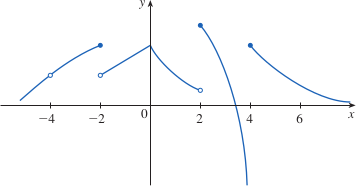
\includegraphics{Images/Image-2.png}    
        \end{center}
        \textbf{Answer: } \\~\\
        \noindent\fbox{
            \parbox{410px}{
                The graph is discontinuous at -4, -2, 2, 4 because f(-4) does not exist and ${\displaystyle\lim_{x \to a} f(x)}$ with $a = -2 \text{, } 2 \text{, } 4$.
            }
          }
        \\
        \item For each of the numbers stated in part (a), determine whether $f$ is continuous from the right, or from the left, or neither.\\
        \textbf{Answer: }\\
        \[ \boxed{{\displaystyle\lim_{t\to -2} f(x)} \text{ is continuous from the left.}}\]\\
        \[ \boxed{{\displaystyle\lim_{t\to 2} f(x)} \text{ is continuous from the right.}}\]\\
        \[ \boxed{{\displaystyle\lim_{t\to 4} f(x)} \text{ is continuous from the right.}}\]\\
    \end{enumerate} 

\end{enumerate}

\newpage
\begin{enumerate}
\setcounter{enumi}{4}
    \item The graph of a function $f$ is given.
    \begin{center}
        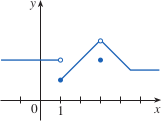
\includegraphics{Images/Image-3.png}
    \end{center}
    \begin{enumerate}
        \item At what numbers $a$ does ${\displaystyle\lim_{t\to a} f(x)}$ not exist?\\
        \textbf{Answer: }\\~\\
        \noindent\fbox{
            \parbox{170px}{
                At 1, ${\displaystyle\lim_{t\to 1} f(x)}$ does not exist.
            }
          }
        \\
        \item At what numbers $a$ is $f$ not continuous?\\
        \textbf{Answer: }\\~\\
        \noindent\fbox{
            \parbox{180px}{
                At 1 and 3, $f$ is not continuous.
            }
          }
        \\
        \item At what numbers $a$ does ${\displaystyle\lim_{x \to a} f(a)}$ exist but $f$ is not continuous at $a$?\\
        \textbf{Answer: }\\~\\
        \noindent\fbox{
            \parbox{280px}{
                At 3, ${\displaystyle\lim_{x \to 1} f(x)}$ exists but $f$ is not continuous at 1.
            }
        }
    \end{enumerate}
\end{enumerate}

\begin{enumerate}
\setcounter{enumi}{12}
    \item Use the definition of continuity and the properties of limits to show that the function is continuous at the given number $a$.
    \[ f(x) = 3x^2 + (x+2)^5 \text{, } a = -1\]
    \textbf{Answer: }\\~\\
    \noindent\fbox{
            \parbox{410px}{
                Because $f(x)$ is a polynomial function, $f(x)$ is continuous on $\mathds{R}$. So it will also be continuous on -1.
            }
        }
\end{enumerate}

\begin{enumerate}
    \setcounter{enumi}{18}
        \item Explain why the function is discontinuous at the given number $a$. Sketch the graph of the function.
        \[ {\displaystyle f(x) = \frac{1}{x+2} \text{ ~ } a = -2} \]
        \textbf{Answer: }\\~\\
        \noindent\fbox{
                \parbox{390px}{
                    Because $f(x)$ is not defined at $x = -2$, so it will not be continuous at $x = -2$.
                }
            }
            \begin{figure}[!h]      
                \begin{framed}
                    \centering  
                \begin{tikzpicture} 
                \begin{axis}[
                    axis lines = center,
                    xlabel = \(x\),
                    ylabel = {\(f(x)\)},
                    xmin=-5, xmax=5,
                    ymin=-10, ymax=10,
                ]
                \addplot [
                    domain=-10:-2.001, 
                    samples=100, 
                    color=red, 
                    ]
                    {1/(x+2)};    
                \addplot [
                    domain=-1.999:10, 
                    samples=100, 
                    color=red, 
                    ]
                    {1/(x+2)};  
                \end{axis}
                \end{tikzpicture}
                \end{framed}
                \end{figure}
\end{enumerate}    

\newpage

\begin{enumerate}
\setcounter{enumi}{24}
    \item Given the equation:
    \[{\displaystyle f(x) = \frac{x-3}{x^2-9}}\]
    \begin{enumerate}
        \item Show that $f$ has a removable discontinuity at $x=3$.\\
        \textbf{Answer: }\\
        $x^2 - 9 \neq 0$\\
        $x = -3 \vee x = 3$\\
        Domain of $f(x)$ is $\mathds{R} \setminus \{-3,3\}$.\\
        \noindent\fbox{
                \parbox{270px}{
                    Therefore, $f(x)$ has a removable continuity at $x = 3$.
                }
            }
        \item Redefine $f(3)$ so that $f$ is continuous at $x=3$ (and thus the discontinuity is “removed”).\\
        
        \[ \boxed{ f(x) = \left \{ \begin{array}{l}
        {\displaystyle \frac{x-3}{x^2-9} \text{ if } x \neq \pm 3} \\
        {\displaystyle \frac{1}{x+3}} \text{ if } x = \pm 3 \end{array} \right. } \]
    \end{enumerate}
\end{enumerate}

\begin{enumerate}
\setcounter{enumi}{26}
    \item Explain, using Theorems 4, 5, 7, and 9, why the function is continuous at every number in its domain. State the domain.
    \[ {\displaystyle f(x) = \frac{x^2}{\sqrt{x^4+2}}}\]
    \textbf{Answer: }\\~\\
    \noindent\fbox{
                \parbox{410px}{
                    Because the function $f$ is a rational function, so it will be continuous at every number in its domain.
                }
            }\\~\\~\\
    $x^4 + 2 > 0$\\
    $x^4 > -2 \text{ (True with all x)}$\\
    \noindent\fbox{
                \parbox{100px}{
                    Domain: $(- \infty, \infty)$
            }\\~\\
    }
\end{enumerate}

\begin{enumerate}
    \setcounter{enumi}{36}
        \item Use continuity to evaluate the limit.
        \[ {\displaystyle \lim_{x \to \frac{\pi}{4}} x^2\tan(x)}\]
        \textbf{Answer: }\\
        $\cos(x) \neq 0$\\~\\
        Domain: ${\displaystyle x \neq \frac{n}{2} + n\pi \text{ with all } n \in \mathds{N}}$\\~\\
        Because $\tan(x)$ is a trignometric function, it will be continuous with all $x$ in its domain.\\
        Moreover, $x^2$ is a polynomial, it will be continuous with all $x$.\\
        Therefore, $f(x)$ will be continuous with all $x$ in its domain.\\~\\
        Because $f(x)$ is continuous, $\boxed{{\displaystyle \lim_{x \to \frac{\pi}{4}} f(x) = f(\frac{\pi}{4}) = 0.6168502751 }}$
    \end{enumerate}

\begin{enumerate}
\setcounter{enumi}{40}
    \item Show that $f$ is continuous on $(- \infty, \infty)$.
        \[ f(x) = \left \{ \begin{array}{l}
    1 - x^2 \text{ if } x \leqslant 1 \\
   \sqrt{x - 1} \text{ if } x > 1 \end{array} \right.  \] 
   \textbf{Answer: }\\
   For $x \neq 1$:\\~\\
        For $x < 1$: $f(x) = 1 - x^2$ is a polynomial, so it will be continuous on the intervals $(-\infty, 1)$.\\
        For $x > 1$: $f(x) = \sqrt{x - 1}$ is continuous on its domain which is $(1, \infty)$.\\~\\
   So, the function will be continuous everywhere except 1. \\~\\
   For $x = 1$:
   \[{\displaystyle \lim_{x \to 1} f(x)}\]
   \[ = \left \{ \begin{array}{l}
    {\displaystyle \lim_{x \to 1^-} (1 - x^2)} = 0 \\
    {\displaystyle \lim_{x \to 1^+} \sqrt{x-1}} = 0 \end{array} \right.  \] \\
    Therefore, ${\displaystyle \lim_{x \to 1^-} (1 - x^2) = \lim_{x \to 1^+} \sqrt{x-1} = \lim_{x \to 1} f(x) = 0 }$.\\~\\
    We also calculate that $f(1) = 0$.\\~\\
    We can conclude that $f(1) = {\displaystyle \lim_{x \to 1} f(x)}$.\\~\\
    \noindent\fbox{
                \parbox{410px}{
                    Since $f(x)$ is already proved to be continuous on $\mathds{R} \setminus \{1\}$, we can conclude that $f(x)$ is continuous on $(-\infty,\infty)$
            }
    }\\~\\
\end{enumerate}

\begin{enumerate}
\setcounter{enumi}{42}
    \item Find the numbers at which $f$ is discontinuous. At which of these numbers is $f$ continuous from the right, from the left, or neither? Sketch the graph of $f$.
    \[ f(x) = \left \{ \begin{array}{l}  
     x^2 \text{ if } x < -1 \\
     x \text{ if } -1 \leqslant x < 1 \\
     {\displaystyle \frac{1}{x} \text{ if } x \geqslant 1} \end{array} \right. \]
    \textbf{Answer: }\\
    For $x = -1$:
        \[{\displaystyle \lim_{x \to -1^-} f(x)}\]
        \[ = {\displaystyle \lim_{x \to -1^-} x^2}\]
        \[ = {\displaystyle \lim_{x \to -1^-} (-1)^2}\]
        \[ = 1 \]\\
        \[{\displaystyle \lim_{x \to -1^+} f(x)}\]
        \[ = {\displaystyle \lim_{x \to -1^+} x}\]
        \[ = -1 \]\\
    Therefore, ${\displaystyle \lim_{x \to -1^-} f(x)} \neq {\displaystyle \lim_{x \to -1^+} f(x)}$, so ${\displaystyle \lim_{x \to -1} f(x)}$ does not exist.\\~\\
    \noindent\fbox{
                \parbox{410px}{
                    Hence, we can conclude that $f(x)$ is discontinuous at $x = -1$. Because if $x = 1$, then $f(x) = x$, we can conclude that $f(x)$ is continuity from the right at $x = 1$
                }
    }\\~\\
    For $x = 1$:
        \[{\displaystyle \lim_{x \to 1^-} f(x)}\]
        \[ = {\displaystyle \lim_{x \to 1^-} x}\]
        \[ = 1 \]
        \\
        \[{\displaystyle \lim_{x \to 1^+} f(x)}\]
        \[ = {\displaystyle \lim_{x \to 1^+} \frac{1}{x}}\]
        \[ = 1 \]\\
    Therefore, ${\displaystyle \lim_{x \to -1^-} f(x)} = {\displaystyle \lim_{x \to -1^+} f(x)}$, so ${\displaystyle \lim_{x \to -1} f(x) = 1}$.\\
    The value of the function at $x = 1$ is: $f(1) = 1$.\\~\\
    \noindent\fbox{
                \parbox{200px}{
                    Therefore, $f(x)$ is continuous at $x = 1$.
                }
    }
    
\begin{figure}[!h]      
    \begin{framed}
        \centering  
    \begin{tikzpicture} 
    \begin{axis}[
        axis lines = center,
        xlabel = \(x\),
        ylabel = {\(f(x)\)},
        xmin=-4, xmax=4,
        ymin=-5, ymax=5,
    ]
    \addplot [
        domain=-10:-1, 
        samples=100, 
        color=red, 
        ]
        {x^2};    
    \addplot [
        domain=-1:1.005, 
        samples=100, 
        color=red, 
        ]
        {x};  
    \addplot [
        domain=1:10, 
        samples=100, 
        color=red, 
        ]
        {1/x};    

    \draw[red, fill=white] (90, 6) circle(1pt);
    \draw[red, fill=red] (90, 4) circle(1pt);

    \end{axis}
    \end{tikzpicture}
    \end{framed}
    \end{figure}

\end{enumerate}

\end{document}

